%=========================================================
% CPU Pipeline Structure
%=========================================================
\section{CPU Pipeline Structure}

For the mmRISC-1 core, the RV32IMAC instruction pipelines consist of 3-stages to 5-stages as shown in Figure \ref{fig:CPUPipeline}.\\\\
Instructions are pre-fetched and queued in the instruction fetch unit which is expressed as “F”, and sent to the next decode stage “D”. Execution stage is shown by “E”, the data memory access stage is “M” and the write back stage is “W”.\\\\

ALU and Integer Multiplication instructions finish at “E” stage, that is, register to register operations are completed in “E” stage.\\\\

Integer Division and Remainder instructions use the non-restoring method and take several clocks to complete.\\\\

Jump instructions generate the target address in the decode stage, and the target address is sent to both the instruction fetch unit and the instruction bus at the next cycle, then the instruction bus gets the code from the instruction memory at “F” stage which is sent to “D” stage at the next cycle of “F”.\\\\

Conditional branch instructions judge whether to take or not to take in “D” stage, and if taken, then follow the same manner as jump instructions. Therefore “D” stage needs register (XRn) forwarding from “E” stage or “W” stage to judge whether to take or not to take.\\\\

Data load instructions generate the access address and send it to the data memory bus at “E” stage. Then, the data bus gets the read data from the data memory at “M” stage, and write back the data to the specified register at “W” stage. If any instruction after the load instruction refers to the loading data (register conflict), the next instruction stalls its “D” stage.\\\\

Data store instructions generate the access address and data to write at “E” stage, and send them to the data memory in “E” stage, then writing to the data memory is completed in “M” stage.\\\\

Detail CPU pipeline logic structure is shown in Figure \ref{fig:CPUPipelineLogicStructure}.\\\\


\begin{figure}[H]
    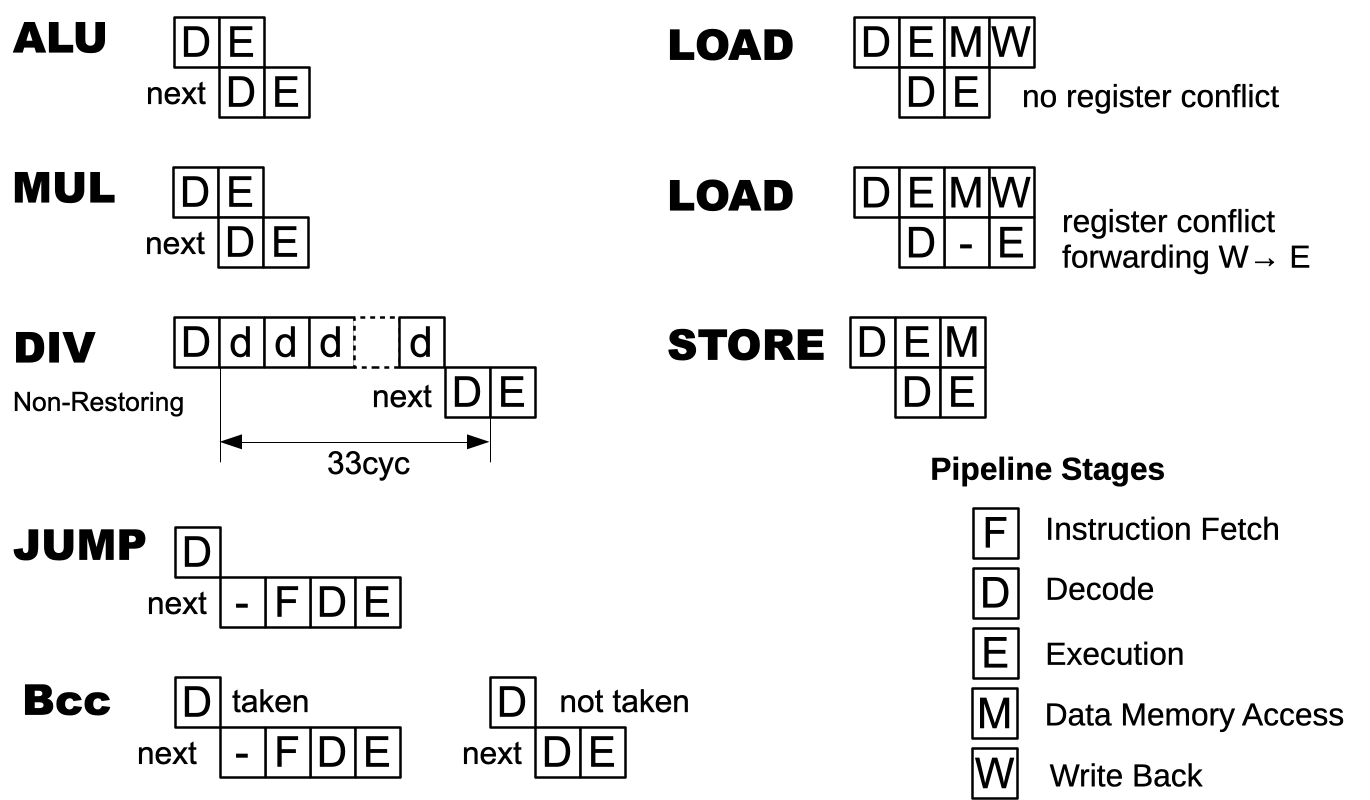
\includegraphics[width=1.00\columnwidth]{./Figure/CPUPipeline.png}
    \caption{CPU Pipeline}
    \label{fig:CPUPipeline}
\end{figure}

\begin{figure}[H]
    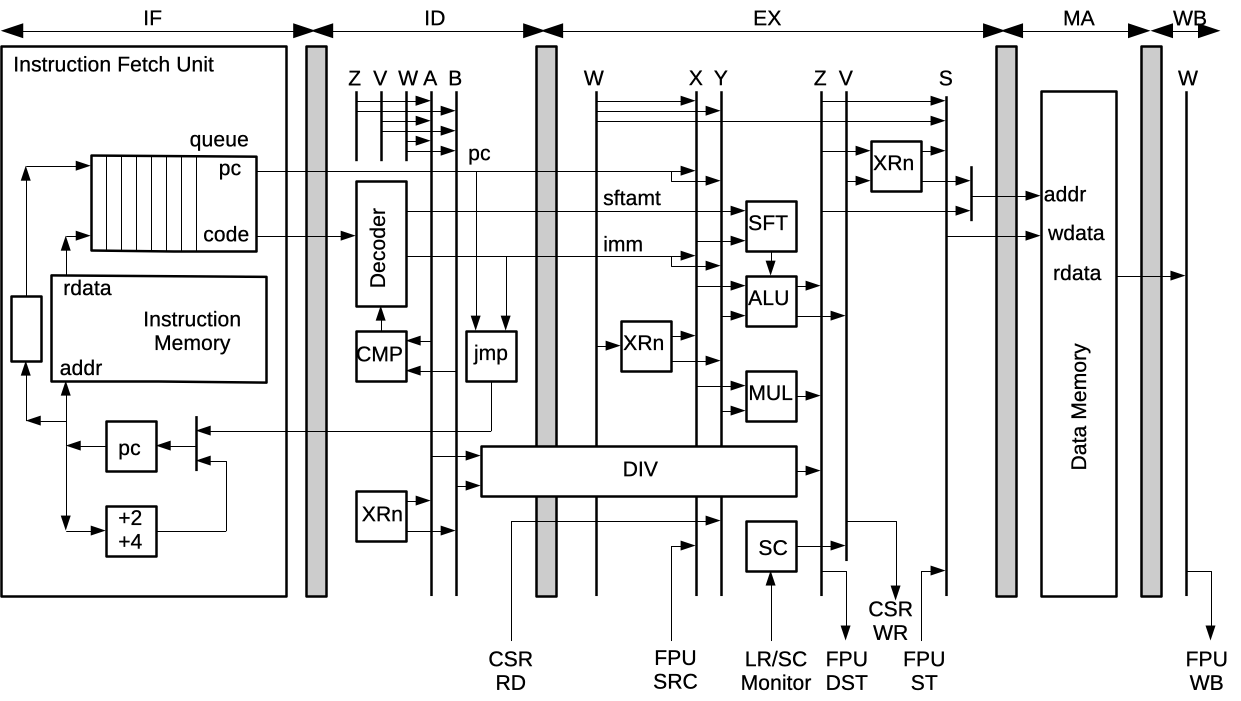
\includegraphics[width=1.00\columnwidth]{./Figure/CPUPipelineLogicStructure.png}
    \caption{CPU Pipeline Logic Structure}
    \label{fig:CPUPipelineLogicStructure}
\end{figure}



